\documentclass[12pt]{article}
\usepackage{tikz}

\usepackage{graphicx, titling, amsmath, amsthm, amsfonts, amssymb, algorithm, algpseudocode}
\usepackage{tikz}

\graphicspath{{./plot1.png/},{./plot2.png/}}

\renewcommand\maketitlehooka{\null\mbox{}\vfill}
\renewcommand\maketitlehookd{\vfill\null}

\title{E0 259 - Assignment 4}
\author{Shankaradithyaa Venkateswaran\\ Sr no: 22190}
\date{\today}

\begin{document}
\begin{titlepage}
    \maketitle
\end{titlepage}

\section{Implementation Summary}
To preprocess the data, I drop all columns except for 'Match', 'Date', 'Innings', 'Over', 'Runs', 'Total.Runs', 'Innings.Total.Runs', 'Runs.Remaining', and 'Wickets.in.Hand'.\\
As given in the instructions, I format the dates correctly and group the data to get all the first innings.\\
Looking through the data, there were some rows with 'Runs.Remaining' as negative. I drop these rows as they are not useful for the analysis.\\
After the preprocessing, I train the model. The template provides the class object for the model with two main methods, 'get\_predictions' and 'calculate\_loss'.\\
I add one more method 'calculate\_loss\_L\_const' which I will explain later.\\
Calling the train\_model function, I initialize the Z0 and L values as 5 and 1 repectively. Now I iterate through all the rows with a common 'Wikets.in.Hand' value and calculate the Z0 and L for each group. I use the Scipy.optimize.minimize function to minimize the loss function provided by the model object.\\
The method that I use is the Nelson-Melder method. I tried using other methods such as Powell, CG, Newton-CG, and trust-constr but they did not converge to the right values. Using these methods led to the predicted values of runs going into the negatives, which led to errors in the log function, and nonsense results at the end. In some cases, the predicted values were NaN.\\
The Nelson-Melder method gave the best results and for the initialization values of Z0 and L as 5 and 1, the outputs are reasonable. The only other method that had somewhat decent results was the BFGS method, which also converged for more initializations. But the final loss was greater than when using Nelson-Melder, hence I stick with Nelson Melder.\\
After getting the Z0 and L values for each group, I take the weighted average of L's according to the instructions given and set the model parameters to the final values.\\
Outside the training function, the model is saved and then the Z0 and L values are printed and plotted.\\
I output a set of 20 parameters along with the model from the training function, and I use these 20 parameters to plot the predicted values of runs for each group.\\
Next, I fix the L value to whatever the weighted average was and optimize over Z0 once more. Here I set the training function flag to false, so that I use the code where L is fixed.\\
In this part of the code, I use the 'calculate\_loss\_L\_const' method to calculate the loss. This method is the same as the 'calculate\_loss' method, but it is structed in such a way that when I pass it through the scipy.optimize.minimize function, it only optimizes over Z0.\\
Here also, I use Nelson-Melder to minimize the loss function.\\
After getting the outputs, I save the model again and plot it with another function called plot\_L\_const. This is the same as the plot function, just that it knows that L is const.\\
I print the 11 parameters as asked and finally calculate the normalized loss.\\
For the normalized loss, I take the final 11 parameters of the model, calculate the loss for all datapoints in the dataset, and then divide by the number of datapoints. I finally report this value.

\section{Results}
\subsection{Plots}
\begin{figure}[h]
    \centering
    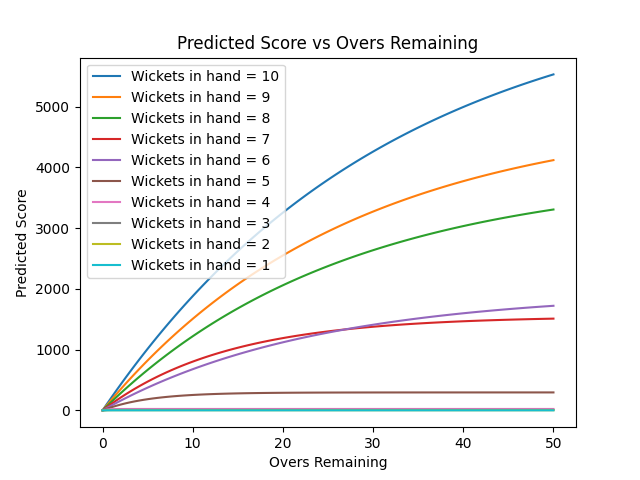
\includegraphics[width=0.8\textwidth]{plot1.png}
    \caption{Plot of Z0 and L values}
\end{figure}
\begin{figure}[h]
    \centering
    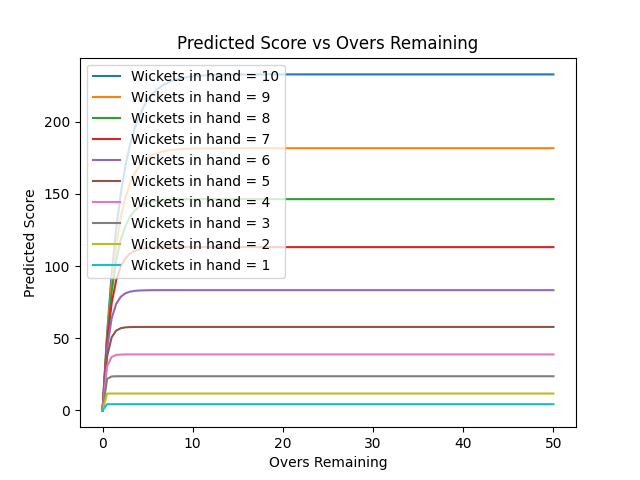
\includegraphics[width=0.8\textwidth]{plot2.png}
    \caption{Plot of Z0 values with L same}
\end{figure}
\subsection{Loss}
Normalised Squared Error Loss = 12.02719457470568
\subsection{Model parameters}
20 parameters from training function:
Z\_0(10) = 6989.08931631325\\
L = 219.11895240734694\\
Z\_0(9) = 4899.63497653183\\
L = 180.13266620990862\\
Z\_0(8) = 3908.5038121186617\\
L = 146.33582994814128\\
Z\_0(7) = 1551.1950508357477\\
L = 113.11575628610183\\
Z\_0(6) = 1953.9654268882412\\
L = 83.29966090290146\\
Z\_0(5) = 295.98369266399106\\
L = 57.822017053092225\\
Z\_0(4) = 23.733258784809554\\
L = 38.771467331110685\\
Z\_0(3) = 9.502122101964638\\
L = 23.65578855845149\\
Z\_0(2) = 3.4893571661283547\\
L = 11.681791458383014\\
Z\_0(1) = 1.343772250546862\\
L = 4.323537596510962\\
After fixing L, 11 parameters:\\
Z\_0(10) = [232.76063071]\\
Z\_0(9) = [181.62392064]\\
Z\_0(8) = [146.34599206]\\
Z\_0(7) = [113.10669037]\\
Z\_0(6) = [83.29830107]\\
Z\_0(5) = [57.82201722]\\
Z\_0(4) = [38.77129993]\\
Z\_0(3) = [23.65508756]\\
Z\_0(2) = [11.680572]\\
Z\_0(1) = [4.32336413]\\
L = 119.52681141591866

\section{Disclaimer}
From the instructions, we were supposed to train the model twice and give two plots. Hence I have changed the arguments to include 2 model files and 2 plots files so that the code can save both outputs.\\
I have also added functions and changed the outputs and inputs of some of them to make my life easier. Overall the structure of the template has been kept the same.\\
Finally, I have used GitHub copilot to help me write the code, I understand I am responsible for the correctness of said code.

\end{document}